\subsubsection{DLL Replacement}
The last missing DLL injection technique of the given attack tree in Figure \ref{fig:attacks_external} is DLL Replacement. The idea is to replace an existing DLL file with a patched or completely different DLL, which is possible due to the windows internal concepts. Every DLL exports functions that can be called from a program. The attacker creates a new DLL file, that exports the same functions and internally redirects all calls to the original DLL file. Therefore the functionality of the application stays the same and the attack is harder to detect. It is now possible to use one of the exported functions to execute other, new code that performs malicious activities.

\subsubsection{\syscall{WriteProcessMemory} external modifications}
\syscall{WriteProcessMemory} is just like the previously discussed \syscall{SetWindowsHookEx} a function available through the Windows API. This function allows to write into the virtual memory of a target process and allows modifying existing data or code. There are several ways to make use of this function, one of them being DLL injection with the \syscall{CreateRemoteThread} and \syscall{LoadLibrary} functions. 

\paragraph{\syscall{CreateRemoteThread} DLL Injection}
DLLs can be loaded into a target process by loading its path into the target memory with \syscall{WriteProcessMemory} and creating a new thread via \syscall{CreateRemoteThread} that calls \syscall{LoadLibrary}. This kind of attack can be used on any process running under the same integrity level and therefore is very widely used in game cheating. At first, a handle to the target process is requested via \syscall{OpenProcess} with \syscall{PROCESS\_VM\_WRITE} and \syscall{PROCESS\_VM\_OPERATION} access rights, which are required to execute the \syscall{WriteProcessMemory} function. If the permissions are missing, \syscall{WriteProcessMemory} is not able to modify the virtual memory of the target process. Virtual memory protection flags do not have to be changed manually, as this is already happening inside \syscall{WriteProcessMemory}. After that, a large enough amount of memory is allocated inside the target process with \syscall{VirtualAllocEx}, to hold the full path of the DLL. Next \syscall{WriteProcessMemory} is used to transfer the DLL path into the target memory space and finally the injection can be completed by calling \syscall{CreateRemoteThread}, which finally loads the DLL with the \syscall{LoadLibrary} function. The allocated memory segment is used as a parameter for the \syscall{LoadLibrary} function call. With the now loaded DLL, arbitrary code can get executed by the DLL, either via using \syscall{CreateRemoteThread} again or via the DLLs entry point.
An example of a basic DLL injection using \syscall{WriteProcessMemory} and \syscall{CreateRemoteThread} can be found in appendix \ref{appendix:writeprocessmemory}. Again, chrome shows no existing defense mechanisms against direct memory modification.

\paragraph{Code modification with \syscall{WriteProcessMemory}}
A second way to make use of \syscall{WriteProcessMemory} is modifying the targets code inside memory, to execute different instructions than intended. This technique is also commonly known as function hooking or function detouring, which is described in the next paragraph. 

\paragraph{Function detouring}
\begin{figure}[!htbp]
	\centering
	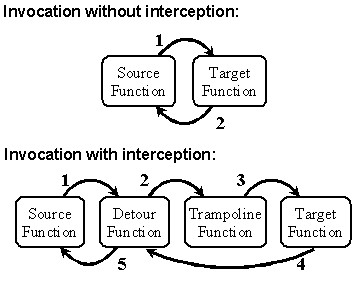
\includegraphics[scale=0.7]{sections/background/attacks/fig_detours.png}
	\caption{This figure shows the change in control flow of a detoured function \cite{detours}}
	\label{fig:detours}
\end{figure}


Function detouring has been greatly simplified by the Detours\cite{msdetours} library of Microsoft, but can also be achieved by memory modification with \syscall{WriteProcessMemory} or assembly code. Figure \ref{fig:detours} shows the difference between a function before and after detouring. The function call at the top shows a invocation without interception. The source function calls the target function without any indirection and after the code of the target function has been executed, returns to the calling source function. Detouring makes use of this structure by placing a detour and a trampoline function in between these calls. The source function will now use an indirect call to the target function, by first calling the detour part, which gives space to execute arbitrary code. To do that, a \syscall{jmp} instruction is placed at the beginning of the function, and the original instructions are saved and copied to the trampoline function. After that, the detour function continues with the trampoline function, which executes the copied instructions and ensures that the target function works as if there was no detour placed. Finally, the whole function stack will return, this time skipping the trampoline function, as it was just used to hold the copied instructions. 

A detection of this technique is very difficult and can only be obtained by measuring the performance of called functions. If execution then takes in average exceptionally longer, there might be a detoured function. It is however impossible to make this detection reliable for all functions, as the systems unexpectable scheduling and load influence the resulting performance.

\subsubsection{Buffer overflows}
Buffer overflows are among the most severe security problems of modern applications, as they are hard to detect, and are introduced by simple programming errors that weren't previously found in testing and quality assurance steps. Even though they are hard to find, once used they allow the attacker to execute arbitrary code. If code execution is not possible, sensitive information might get revealed. One of the most severe examples of the past was the so called "Heathbleed bug", which affected millions of servers worldwide, as it was present in the much used OpenSSL library. Even though the attacker couldn't execute code, he was able to get sensitive information about the SSL certificates private key and thus break any security put in place by the SSL protocol. This attack is the last one of Figure \ref{fig:attacks_external} and also a external modification. In contrast to the other previously shown attacks there are several countermeasures existing to mitigate the resulting exploit, which will be discussed in chapter \ref{sec:defenses}.

\subsubsection{Internal modifications}
\label{sec:internal_modifications}
\begin{figure}[h]
\centering
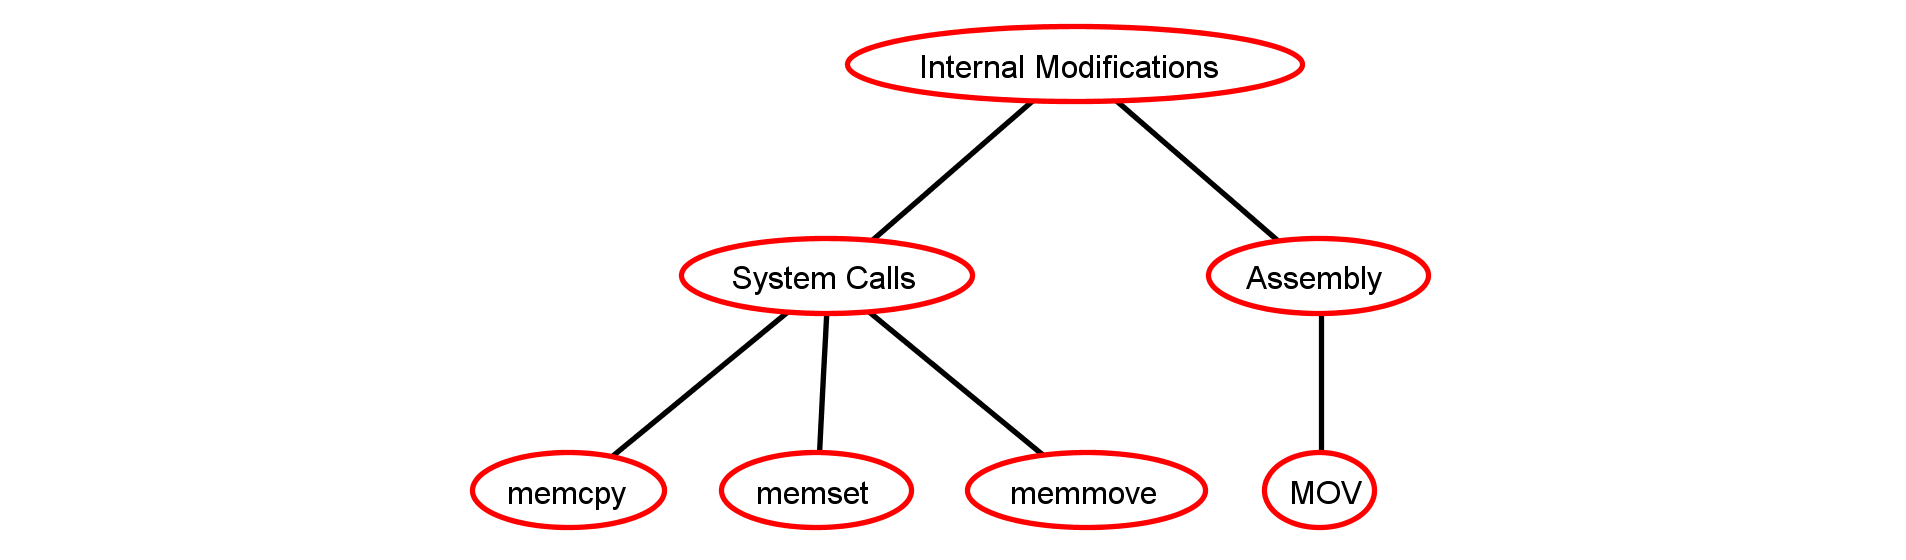
\includegraphics[scale=0.45]{sections/adtrees/InternalModificationsWithoutDefenses.png}
\caption{This attack tree shows possible attacks that are grouped under internal modification}
\label{fig:attacks_internal}
\end{figure}
A group of attack is internal modifications which is in contrast to external modifications occurring from inside the process virtual memory. As the attacker is already inside the virtual memory, modification is easier and less restricted then the previously shown external modifications. The attacker can make use of existing functions like \syscall{memcpy} or \syscall{memset}, to modifiy the values inside memory, without having to use the indirection via \syscall{WriteProcessMemory}. Besides the present \syscall{mem*} functions, the attacker can also make use of assembly code. Figure \ref{fig:attacks_internal} shows this type of attack. The assembly part outlines the \syscall{mov} instruction, as it is mainly used to detour functions without the usage of exported API functions.